\documentclass[11pt]{article}


\usepackage{amsfonts}
\usepackage{fancyvrb}
\usepackage{graphicx}
\usepackage{caption}
\usepackage{subcaption}
\usepackage{url}

\setlength{\oddsidemargin}{0in}
\setlength{\evensidemargin}{0in}
\setlength{\textwidth}{6.5in}
\setlength{\topmargin}{0in}
\setlength{\headsep}{0.5in}
\setlength{\textheight}{8.5in}
\setcounter{page}{1}
%\pagestyle{empty}
%\hbadness=10000

\begin{document}
\huge
\noindent
{Discrete Optimization Assignment:}
\vspace{0.25cm}

\noindent
{\bf Traveling Salesman Problem}
\normalsize


\section{Problem Statement}

In this assignment you will design an algorithm to solve a fundamental problem faced by every traveling salesperson, aptly named {\em The Traveling Salesman Problem (TSP)}.  All traveling salespeople start from their home, travel to several cities to sell their goods, and complete the day by returning home.  To minimize their costs, traveling salespeople strive to visit all of the cities using the shortest total travel distance.  This amounts to finding a visitation order of all of the cities that  minimizes the sum of distances traveled when moving from one city to another.  Figure \ref{fig:tsp} illustrates a small TSP and a feasible solution to that problem.  The cities are labeled from $0..4$.


\begin{figure}[h]
        \centering
        \begin{subfigure}[b]{8.0cm}%{0.3\textwidth}
                \centering
                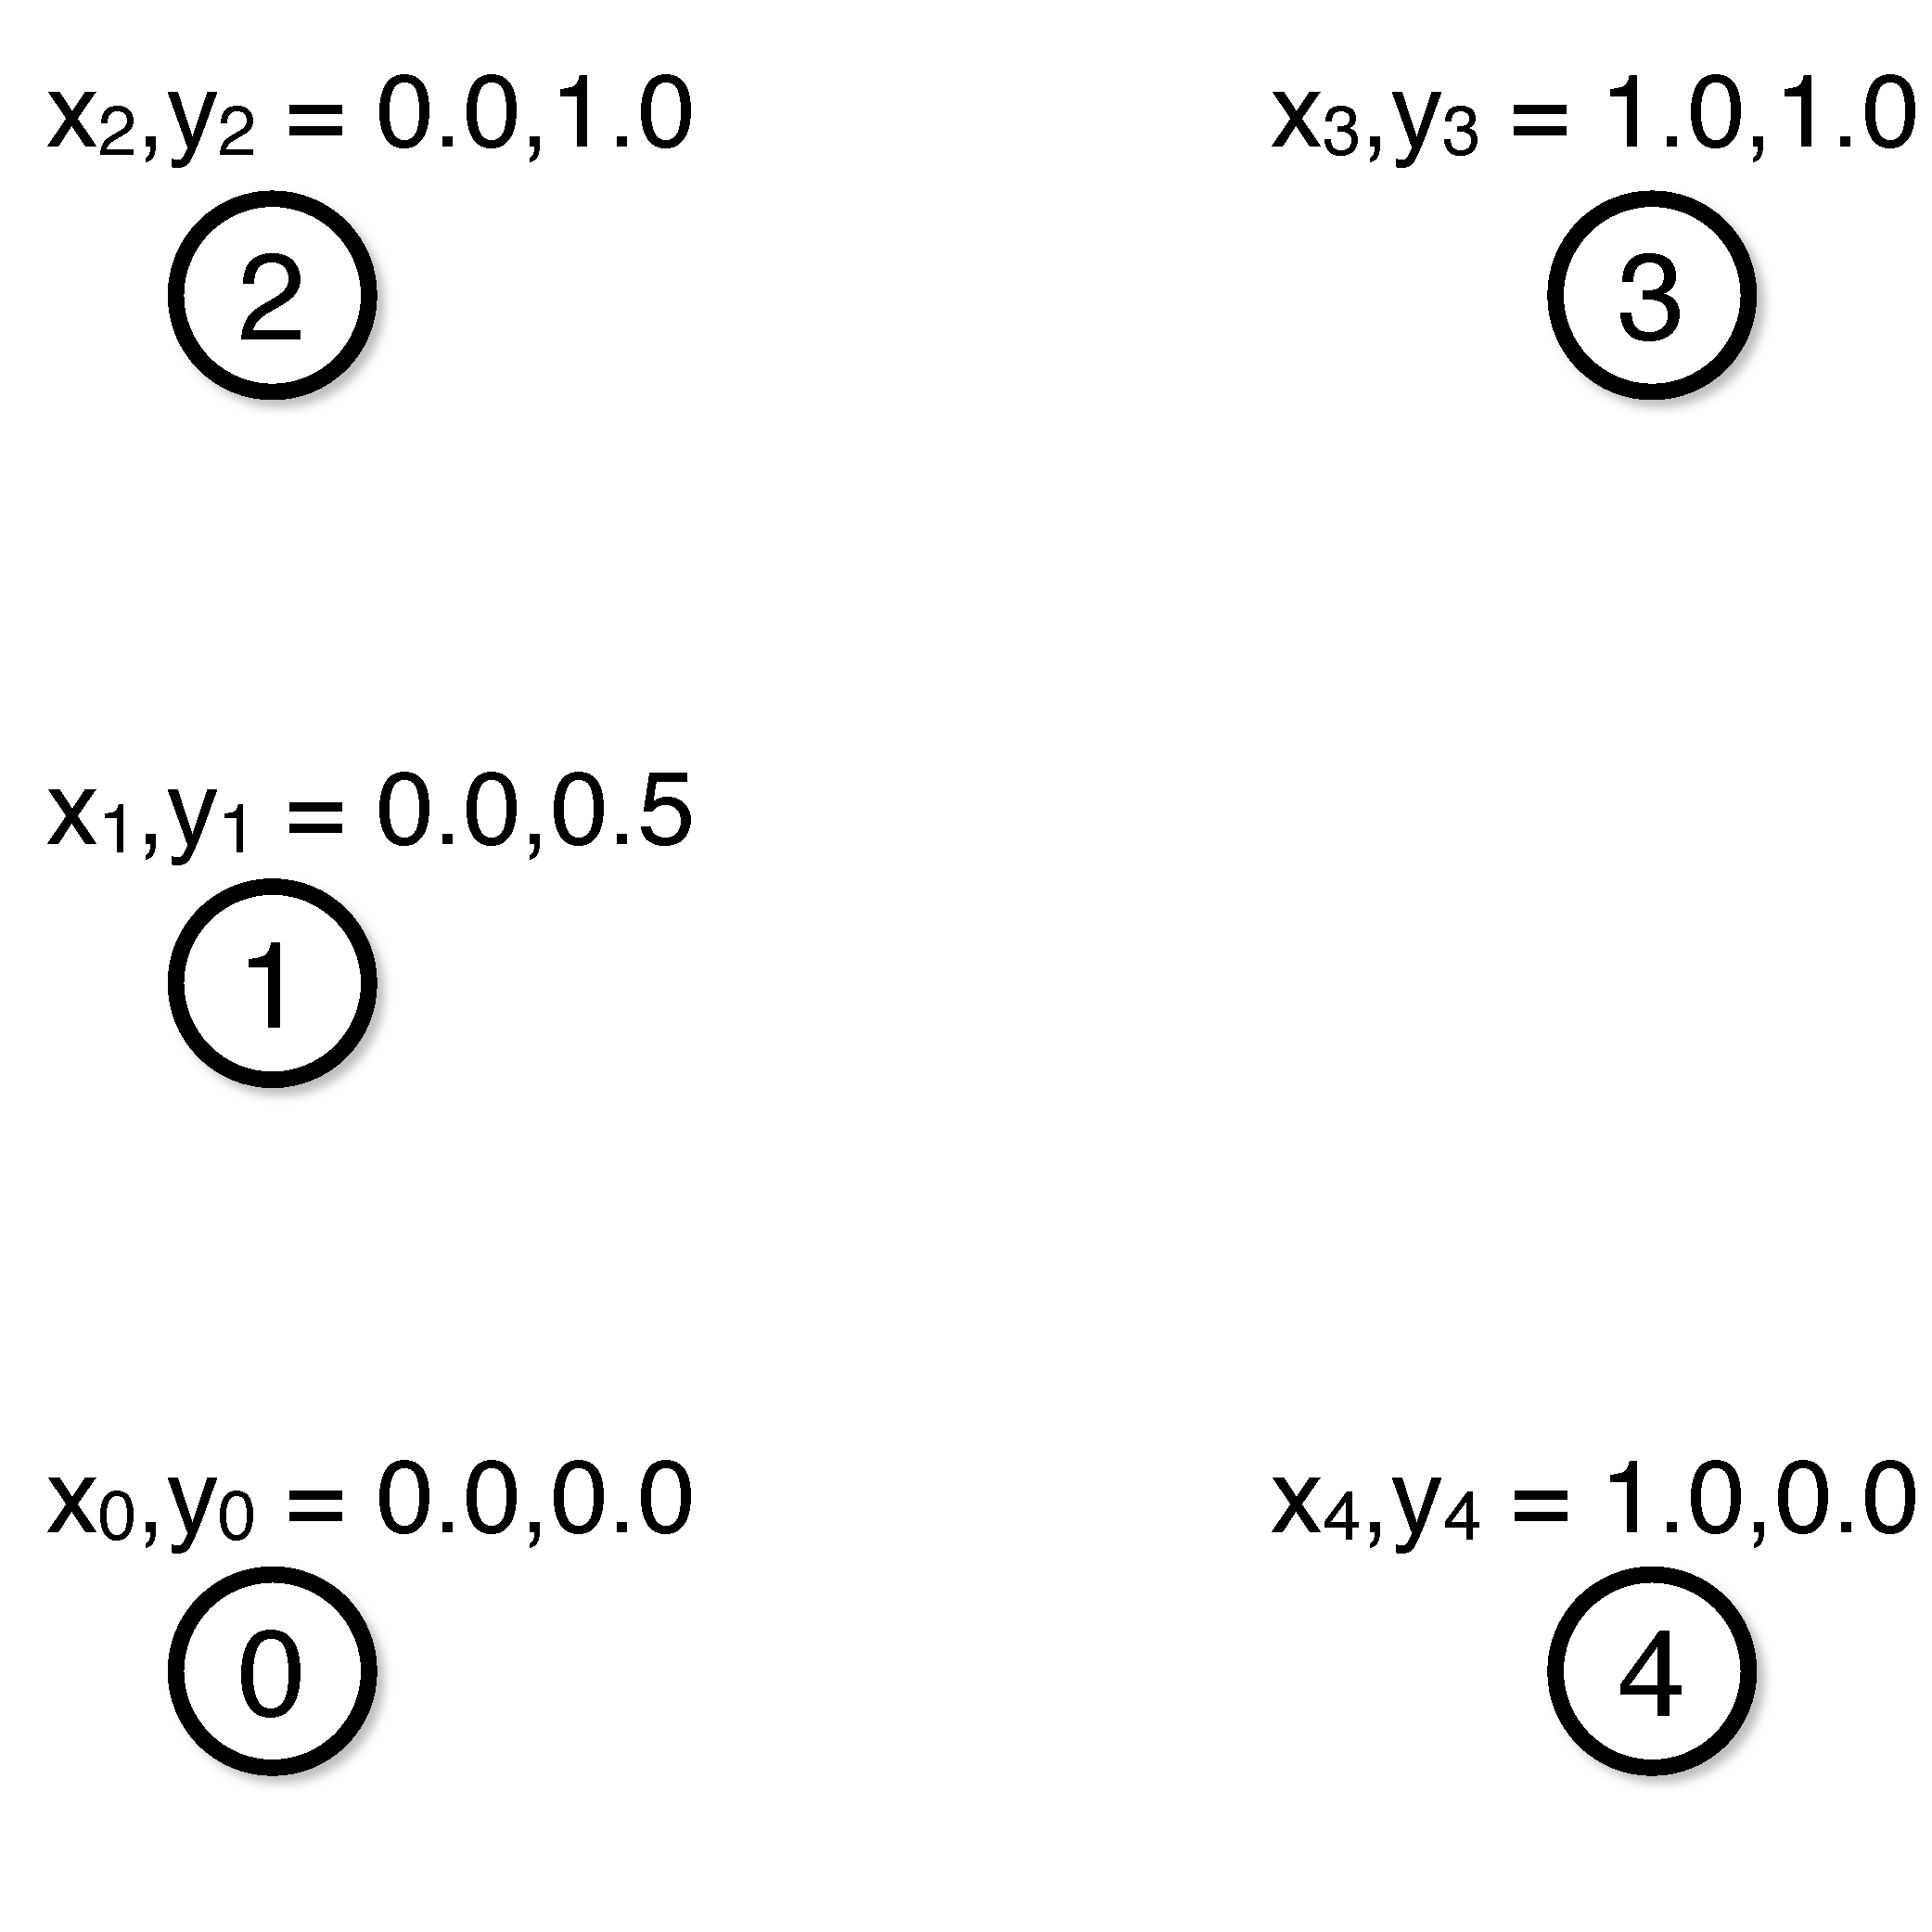
\includegraphics[width=6cm]{figures/tsp_1.pdf}
                \caption{The TSP input data.}
                \label{fig:vrp:input}
        \end{subfigure}%
        ~ %add desired spacing between images, e. g. ~, \quad, \qquad etc.
          %(or a blank line to force the subfigure onto a new line)
        \hfill
        \begin{subfigure}[b]{8.0cm}
                \centering
                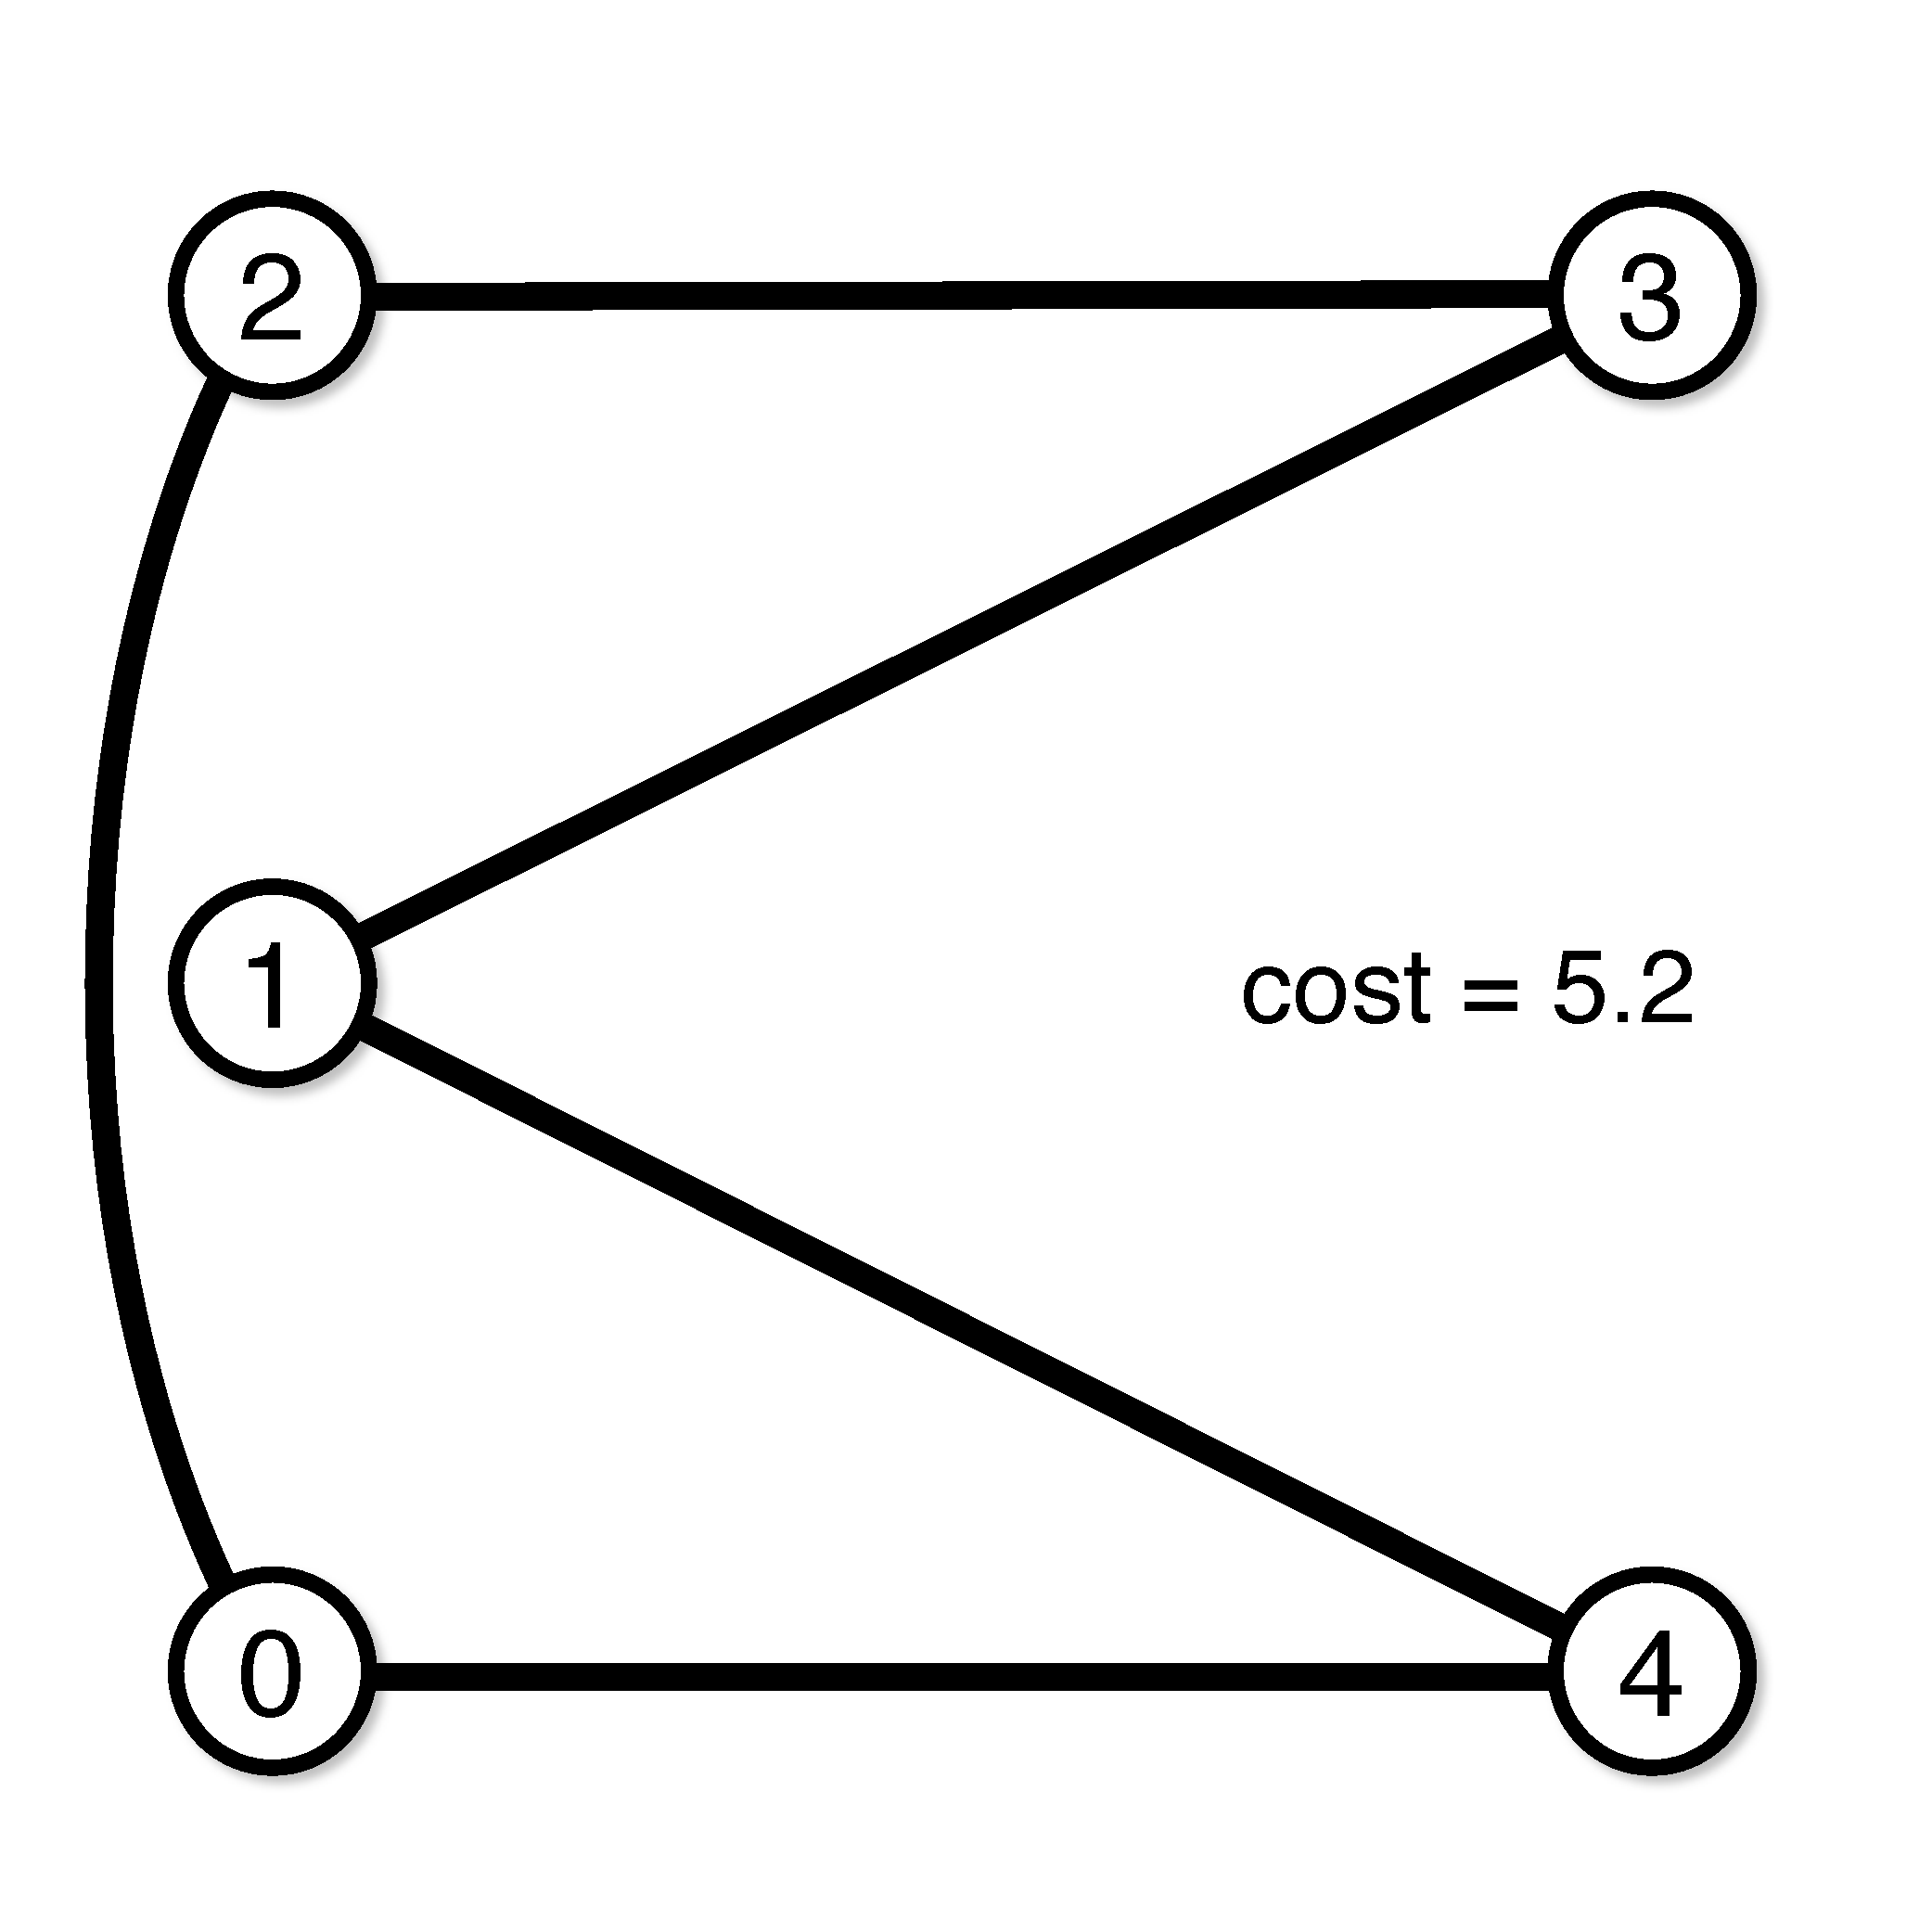
\includegraphics[width=6cm]{figures/tsp_2.pdf}
                \caption{A solution to the TSP.}
                \label{fig:vrp:sol}
        \end{subfigure}
        \caption{A Traveling Salesman Example}\label{fig:tsp}
\end{figure}

\section{Assignment}

Write an algorithm to solve the traveling salesman problem (a.k.a. minimize the length of a hamiltonian cycle\footnote{See \url{http://en.wikipedia.org/wiki/Hamiltonian_path}} of a graph).  The problem is mathematically formulated in the following way:  Given a list of locations $N = 0 \ldots n-1$ and coordinates for each location $\langle x_i,y_i \rangle \; i \in N$.  Let $v_i \;\; i \in N$ be a variable denoting the visitation order (i.e. the value of $v_i$ is the $i$-th location to be visited) and let ${\it dist}(l_1,l_2)$ be the Euclidean distance between two locations.\footnote{${\it dist}(n,m) = \sqrt{(x_{n} - x_{m})^2 + (y_{n} - y_{m})^2}$}  Then the traveling salesman problem is formalized as the following optimization problem,
$$
\begin{array}{ll}
\mbox{minimize:} & \displaystyle \sum_{i \in 0 \ldots n-1} dist(v_i,v_{i+1}) + dist(v_n,v_{0}) \\
\mbox{subject to:} & \\
     & v_i\mbox{ are a permutation of } N 
\end{array}
$$
In this variant of the traveling salesman problem, we assume the sales person travels by helicopter and can go directly in a straight line from one point to another.

\section{Data Format Specification}

The input consists of $|N| + 1$ lines.  The first line contains one number $|N|$.
It is followed by $|N|$ lines, each line represents a point $\langle x_i, y_i \rangle$ where $x_i, y_j \in \mathbb{R}$.

\vspace{0.2cm}
\noindent
Input Format
\vspace{-0.2cm}
\begin{Verbatim}[frame=single]
|N| 
x_0 y_0
x_1 y_1
...
x_|N|-1 y_|N|-1
\end{Verbatim}
%
The output has two lines.  The first line contains two values $obj$ and $opt$.  $obj$ is the length of the hamiltonian cycle (i.e. the objective value) as a real number.  $opt$ should be $1$ if your algorithm proved optimality and $0$ otherwise.  The next line is a list of $n$ values in $N$, one for each of the $v_i$ variables.  This line encodes the solution.

\vspace{0.2cm}
\noindent
Output Format
\vspace{-0.2cm}
\begin{Verbatim}[frame=single]
obj opt
v_0 v_1 v_2 ... v_|N|-1
\end{Verbatim}
%
%It is essential that the value order in the solution output matches the value order of the input.  Otherwise the grader will misinterpret the output.

\paragraph{Examples} \mbox{}
%\vspace{0.1cm}
%\noindent
(based on Figure \ref{fig:tsp})

\vspace{0.2cm}
\noindent
Input Example
\vspace{-0.2cm}
\begin{Verbatim}[frame=single]
5
0 0
0 0.5
0 1
1 1
1 0
\end{Verbatim}

\vspace{0.2cm}
\noindent
Output Example
\vspace{-0.2cm}
\begin{Verbatim}[frame=single]
5.2 0
0 4 1 3 2
\end{Verbatim}
%
This output represents the following hamiltonian cycle, $\{0 \rightarrow 4, 4 \rightarrow 1, 1 \rightarrow 3, 3 \rightarrow 2, 2 \rightarrow 0\}$

\section{Instructions}

Edit \texttt{solver.py} and modify the \texttt{solve\_it(input\_data)} function to solve the optimization problem described above.  The function argument, \texttt{input\_data}, contains the problem data in the format described above.  The return value of \texttt{solve\_it} is a solution to the problem in the output format described above.  Your \texttt{solve\_it} implementation can be tested with the command, 
\[ 
\texttt{python ./solver.py ./data/<inputFileName>} 
\] 
You should limit the \texttt{solve\_it} method to terminate within 5 hours, otherwise the submission will not be eligible for full credit.  You may choose to implement your solver directly in python or modify the \texttt{solve\_it} function to call an external application.

%We use \texttt{stdout} for output.
%Output to other stream will be ignored (you may want to send runtime information to \texttt{stderr}). Your submission will be tested on a department linux machine. If your algorithm is a standalone program, please name it \texttt{nr},
%otherwise, please specify the compilation procedure,
%it is appreciated if you also provide a script that follows the above format to run the program.

\paragraph{Resources}
You will find several  traveling salesman problem instances in the \texttt{data} directory provided with the handout.

%An example output file, \texttt{blabla.out}, is also provided.

%\section{Remarks}

\paragraph{Handin}
Run \texttt{submit.py} with the command, \texttt{python ./submit.py}.  Follow the instructions to apply your  \texttt{solve\_it} method on the various assignment parts.  You can submit multiple times and your grade will be the best of all submissions.  However, it may take several minutes before your assignment is graded; please be patient.  You can track the status of your submission on the {\em feedback} section of the assignment website.


\paragraph{Grading}
Infeasible solutions (i.e. those that do not conform to the output format or violate problem constraints) will receive 0 points.  Feasible solutions will receive at least 3 points.  Feasible solutions passing a low quality bar will receive at least 7 points and solutions meeting a high quality bar will receive all 10 points.  The grading feedback indicates how much your solution must improve to receive a higher grade.


\paragraph{Collaboration Rules} 

In all assignments we encourage collaboration and the exchange of ideas on the discussion forums.  However, please refrain from the following:
\begin{enumerate}
\item Posting code or pseudo-code related to the assignments.
\item Using code which is not your own.
\item Posting or sharing problem solutions.
\end{enumerate}
Discussion of solution quality (i.e. objective value) and algorithm performance (i.e. run time) is allowed and the assignment leader board is designed to encourage such discussions.


%\paragraph{Questions} Please contact the class GTA Carleton (cjc@cs.brown.edu).

\paragraph{Warnings} 

\begin{enumerate}
\item It is recommended you do not modify the \texttt{data} directory.  Modifying the files in the data directory risks
making your assignment submissions incorrect.
\item You cannot rename the \texttt{solver.py} file or the \texttt{solve\_it()} method.
\item Be careful when using global variables in your implementation.  The \texttt{solve\_it()} method will be run repeatedly and it is your job to clear the global data between runs.
\item \texttt{solver.py} must remain in the same directory as \texttt{submit.py}.
\end{enumerate}


%\paragraph{Hint} 
%The optimal value for  \texttt{data/gc\_1000\_5} is near $85$.
 
\section{Technical Requirements}

You will need to have python 2.7.x or 3.5.x installed on your system (installation instructions, \\ \texttt{\url{http://www.python.org/downloads/}}).


\end{document}




